\documentclass[output=paper]{langsci/langscibook}
\ChapterDOI{10.5281/zenodo.1407021}

\hyphenation{obj-exp}
\hyphenation{-ment}





\title{A frame-semantic approach to polysemy in affixation}
\author{Ingo Plag\and Marios Andreou\lastand Lea Kawaletz\affiliation{University of Düsseldorf}}

\abstract{One of the central problems in the semantics of derived words is \isi{polysemy}. The most advanced theory of \isi{derivational semantics} to date is the Lexical Semantic Framework developed by  %
%Lieber (2004 et seq.)
\citeauthor{Lieber.2004} (\citeyear{Lieber.2004} et seq.)%
%\citet[et seq.]{Lieber.2004}%
%Lieber
%
. This theory, however, does not have a straightforward answer to the question of which kinds of meaning extensions\is{meaning extension} are possible and which ones should be impossible for a given derivative. This is all the more so for deverbal derivation, where Lieber explicitly leaves open exactly what the `semantic body' of verbs, i.e. (roughly) the encyclopedic and cultural knowledge involved in interpretation, looks like \citet[72]{Lieber.2004}).

This paper tackles this problem by putting forward a new formal approach to \isi{derivational semantics}, i.e. frame semantics. In frame theory (\citealt{Barsalou.1992a, Barsalou.1992b}, \citealt{Lobner13}), frames are complex structures which model mental representations of concepts. These representations are typed, recursive attribute-value structures, where the attributes are functional relations, assigning unique values to the concept they describe (see \citealt{Petersen.2007}). Using the apparatus of this framework, we hypothesize that the semantics of a derivational process\is{derivational semantics} is describable as its potential to perform certain operations (such as metonymic shifts) on the frames of its bases.

We propose a particular  model of affixal polysemy\is{polysemy!affixal polysemy} in which attested readings of words of a given morphological category result from indexation of particular elements of the frame-semantic representation, combined with \isi{inheritance} mechanisms. For deverbal nominalizations in English \textit{-ment}, the shifts can target (syntactically) argumental and non-argumental components. Different bases thus go along with different kinds of semantic shifts in their derivatives.  Given a particular verb class, possible readings of the respective derivatives are predictable.}


\maketitle

\begin{document}
\selectlanguage{english}
\is{frame semantics|(}
\il{English|(}
\is{polysemy!affixal polysemy}
\is{polysemy}

\section{Introduction}

In many languages \isi{polysemy} in word-formation is all-pervasive (e.g. \citealt{Rainer.2014c}). Following %
%Bauer et al. (2013)
\citet{Bauer.2013}%
%Bauer-al.
%
, \citet[291]{Kawaletz.2015} list a number of readings of English deverbal nominalizations involving the suffixes \textit{-ing, -ation, -ment, -ance/-ence, -th} and conversion, as given in Table \ref{tab:English}.


\begin{table} 
\fittable{
    \begin{tabular}{lll}
	    \lsptoprule
	    {Semantic category} & {Paraphrase} & {Examples} \\
	    \midrule
    Event & `the event of V-ing' &  \textit{production, training}\\
    Result & `the outcome of V-ing' &  \textit{acceptance, alteration}\\
    Product & `the thing that is created by V-ing' &  \textit{pavement, growth}\\
    Instrument & `the thing that V-s' &  \textit{seasoning, advertisement}\\
    Location & `the place of V-ing' &  \textit{dump, residence}\\
    Agent & `people or person who V-s' &  \textit{administration, cook}\\
    Measure & `how much is V-ed' & \textit{ pinch, deceleration}\\
    Path & `the direction of V-ing' &  \textit{decline, direction}\\
    Patient & `the thing affected or moved by V-ing' &  \textit{catch, acquisition}\\
    State & `the state of V-ing or being V-ed' &  \textit{alienation, disappointment}\\
    Instance & `an instance of V-ing' & \textit{belch, cuddle} \\
    \lspbottomrule
\end{tabular} 
}
  \caption{Readings of English nominalizations \citep{Kawaletz.2015}}
  \label{tab:English}
\end{table}

For other languages, similar lists have been produced. For example, for \ili{French} we find the data shown in Table \ref{tab:French} in \cite{Fradin.2012b} (see also, for example, \citet{Uth.2011}, \citet{Fradin.2011}, \citet{Fradin.2012a} for \ili{French}, \citet{Rossdeutscher.2010}, \citet{Rossdeutscher.2010b} for German).

\begin{table}  
	 
\begin{tabularx}{\textwidth}{Xlll}
	\lsptoprule
	{Semantic category} & {Paraphrase} & {Example} & {Translation}\\
	\midrule
	Event & `action of V-ing'  & \textit{lavage}  & `washing'\\
	Product  & `resulting object'  & \textit{construction}  & `building'\\
	Means   & `what Vs'  & \textit{emballage}  & `wrapping'\\
	State  & `fact of being Ved' &  \textit{embrouillement}  &  `muddle'\\
	Manner & `manner of V-ing'  & \textit{marche}  & `gait'\\
	Location  & `place where one V-s'  &  \textit{garage} &  `garage'\\
	Group  &  `people who V'  & \textit{\'{e}quipage}  & `crew'\\
	Period  & `time during which one V-s'  & \textit{hivernage}  & `wintering'\\
	\lspbottomrule
\end{tabularx} 
\caption{Readings of \ili{French} nominalizations \citep{Fradin.2012b}}
\label{tab:French}
\end{table}

These facts raise a number of very general questions. Do affixes have meaning, and if so, how can we describe this meaning? Given the variety of interpretations that derivatives of a given affix can give rise to, this does not seem to be a trivial task. Which kinds of readings or \isi{meaning extension} are possible and which ones should be impossible for a given derivative? How does the meaning of the base interact with the meaning of the affix? What are the principles or mechanisms that account for this interaction? In spite of the growing number of studies in this domain the answers to these questions are still under debate and we are still facing the task of accounting ``for the substantial evidence that affixes [...] are frequently semantically underspecified, and subject to \isi{polysemy} and meaning extensions\is{meaning extension} of various sorts" \citep[641]{Bauer.2013}.

The crucial question is how the different readings of a given derivative emerge, and, as a result, how the different readings of different derivatives of a particular morphological category come about. Some generalizations have been proposed that give at least partial answers to these questions. For example, authors like \citet[212]{Bauer.2013} have claimed that certain base verbs evoke certain readings in the nouns derived from them, but systematic studies exploring this claim in more detail and with larger amounts of data are rare. Hence, \citet[213]{Bauer.2013} only list a few potential generalizations, for example that state nominalizations frequently derive from verbs of psychological state, and that verbs with inherently spatial denotations give rise to location nominalizations.

With regard to \ili{French}, \cite{Ferret.2013} and \cite{Ferret.2015} hold that specific readings of derived nouns only arise ``if very specific semantic conditions are met by the base verb" \citep[480]{Ferret.2015}. In the case of instrument readings with nouns in \textit{-oir} or \textit{-age}, this reading can only occur if the base verb denotes an externally caused event which involves an instrumental semantic participant.

What is perhaps noteworthy at this point is the fact that deverbal nominalizations can not only lexicalize the event denoted by the verb or the verb's syntactic arguments, but also other entities that are part of the semantic representation of the base verb. For illustration consider (\ref{ex:purchase}). In (\ref{ex:purchase}a) we find an eventive interpretation of the converted noun \textit{purchase}, while in (\ref{ex:purchase}b) there is an object argument reading (`the thing that was purchased'). Similarly, (\ref{ex:embroidery}a) shows an eventive reading, but, as shown in (\ref{ex:embroidery}b), also other things can be profiled. Thus an \textit{embroidery} is not the thing that is embroidered (i.e the internal argument of the verb), but the entity that results from the activity of embroidering.


\begin{exe}
	\ex \label{ex:purchase}
	\begin{xlist}
		\ex  {}[S]earching through the store to find someone to help, I completed my \emph{purchase} and then went home feeling dismissed (COCA NEWS 1998)
		\ex Outside the store I deposited my \emph{purchase} in a trash can. (COCA FIC 2008)
		\end{xlist}
	\ex \label{ex:embroidery}
	\begin{xlist}
		\ex Her daughter Daphne wisely made no comment and pretended to be engrossed in her \emph{embroidery}. (COCA FIC 2000)
		\ex {}[T]he nails of her feet and hands matched the color of the \emph{embroidery} of her leine. (COCA FIC 2010)
	\end{xlist}
\end{exe}

In this paper we will introduce a new approach to the formalization of the interpretation of derived words based on frames and apply this approach to the analysis of \textit{-ment} derivatives that are based on change-of-state verbs and psych verbs.

\section{The framework: Frame semantics}

The approach adopted in the present paper builds on predecessors in cognitive science and artificial intelligence such as Marvin \citegen{Minsky1975} frame theory, the schema theory of \citet{Bartlett.1932}, and, specific to linguistics, Fillmore's work on situation frames (\citealt{Fillmore.1982}; see \citealt{Busse.2012} for a historical overview of the development of frame semantics). We use the notion of `frame' in the specific sense of \citet{Barsalou.1992a, Barsalou.1992b}, \citet{Petersen.2007} and \citet{Lobner13}. In this framework, frames are recursive attribute-value structures as known from other frameworks (e.g. HPSG, \citealt{Pollard94}). Frames are taken to be a general format of mental representations of concepts which is also applicable to linguistic phenomena. Frames can be depicted as graphs with nodes and arcs, or as attribute-value matrices, as shown for the toy example \textit{John hit the ball} in Figure \ref{fig:frames}, with the graph on the left and the attribute-value matrix on the right.

%\begin{multicols}{2}

\begin{figure}
		\centering
		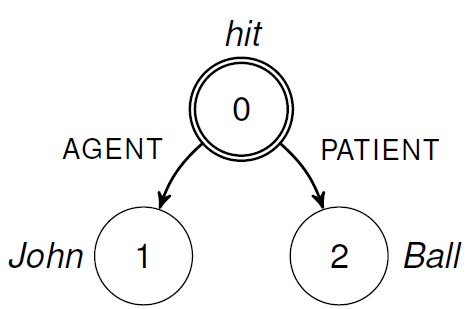
\includegraphics[scale=0.25]{figures/PlagAndreouKawaletz-hit2.png}
		\hspace*{3em}
		\begin{tabular}[b]{l}
		\begin{avm}
		\@0 \[\asort{hit} agent & \@1 John\\ patient & \@2 Ball\]
		\end{avm}
		\\ \\
		\end{tabular}
\caption{Two ways of depicting a frame}
\label{fig:frames}
\end{figure}

In both representations the referential node, which represents the event as a whole, is labeled \textit{hit} (marked by a double circle in the graph), and this hitting event has two attributes (which, in this case, stand for the participants), an \textsc{agent} attribute with the value \textit{John} and a \textsc{patient} attribute with the value \textit{ball}. Entities in graphs and matrices are often indexed for ease of reference (for example with {\avmbox{0}, \avmbox{1} and \avmbox{2}}, as in the attribute-value matrix).

In this approach, attributes are functional in the mathematical sense. The attribute-value structures are recursive and they allow for structure sharing (identities of attribute values). The values by which an attribute can be specified are subordinate concepts of this attribute (\citealt[43]{Barsalou.1992b}). In Petersen's frame approach, the resulting taxonomy is incorporated in the type signature underlying each frame (cf. \citealt[Def. 8 and Fig. 9]{Petersen.2007}).

Returning to the problem of verbal bases, our formalism can be used to depict the semantic representation of specific verb classes. For illustration consider a class that is frequently discussed in the literature and that is also a possible base for \textit{-ment} derivation, change-of-state verbs (e.g. \citealt{Levin.1993}, \citealt{Levin.1995}, \citealt{RappaportHovav.1998}, \citealt{Dowty.1979}, \citealt{Pustejovsky.1991}, \citealt{vanValin.1997}, \citealt{Alexiadou.2015}). According to many analyses, causation events as expressed by change-of-state verbs (such as \textit{break}) are complex events that consist of two sub-events, a cause and an effect. In a frame semantic analysis, causation events can be formalized as in Figure \ref{fig:cosation}.

\begin{figure}

		\begin{avm}

		\@0	\[\asort{causation event}
			\textsc{actor} & \@1 \cr
			\textsc{undergoer} & \@2 \cr
			\textsc{instrument}  & \@3 \cr

			\textsc{cause} & \@4 \[ \asort{activity} 
			\textsc{actor} & \@1 \cr
			\textsc{undergoer} & \@2 \cr
			\textsc{instrument} & \@3 \cr
			\] \cr
			\textsc{effect} & \@5 \[ \asort{change-of-state} 
			\textsc{initial state} & \@6 \[ \asort{state} 
			\textsc{patient} & \@2\cr
			\]\cr
			\textsc{result state} & \@7 \[ \asort{state} 
			\textsc{patient} & \@2\cr
			\] \cr
			\]\cr
			\]
	\end{avm}
	\caption{Change-of-state verbs}
	\label{fig:cosation}
	
\end{figure}

Figure \ref{fig:cosation}  depicts a typical \textit{change-of-state} verb. The representation is based on established semantic roles (e.g. \textsc{actor, undergoer}) in combination with an event frame. In other words, it combines the participants typically associated with such verbs, and embeds them in the event structure assumed for externally caused events.

A change-of-state verb has three core participants: \textsc{actor (\avmbox{1}), undergoer (\avmbox{2})} and, quite often, an \textsc{instrument} (\avmbox{3}). One of the two sub-events, \textsc{cause} (\avmbox{4}) consists of an \textit{activity} with the same three participants.  The \textsc{cause} sub-event is typically an \textit{activity}, but could also be any other type of event. The activity has an \textsc{effect} (\avmbox{5}), which constitutes the second sub-event, which is a \textit{change-of-state}. The \textit{change-of-state} involves an \textsc{initial state} (\avmbox{6}) and a \textsc{result state} (\avmbox{7}) of a \textsc{patient}. 
%The \textsc{result state} must not be identical to the initial one, which is formalized by the unequal sign between the two indices at the bottom of the matrix. 
The \textsc{patient} of the two states is the \textsc{undergoer} of the event \avmbox{0}.

Another verb class that is very common as a base for \textit{-ment} derivatives is that of psych verbs. The use of the term `psych verb' is not consistent in the literature, and different authors define this class differently. We use the term in this paper as referring to so-called `object experiencer verbs'. These are verbs (such as \textit{amuse}) where the subject denotes the stimulus, and the object denotes the experiencer in an event in which the experiencer undergoes a change in its psychological state (see, for example, \citet [189] {Levin.1993} for discussion). Psych verbs can thus be considered a sub-class of change-of-state verbs, and they are also referred to as `psych causation' verbs. A frame-semantic representation of such verbs is given in Figure \ref{fig:psych}.

\begin{figure}
	
\begin{avm}
	\@0 \[ \asort{psych causation}
	\textsc{stimulus} & \@1 \cr
	\textsc{experiencer} & \@2 \cr
	\textsc{cause} & \[ \asort{activity}
	\textsc{actor} & \@1 & \cr
	\textsc{undergoer} & \@2 \cr
	\] \cr
	\textsc{effect} & \[ \asort{change-of-psych-state} 
	\textsc{initial state} & \@3 & \[ \asort{psych state}
	\textsc{experiencer} & \@2\cr
	\]\cr
	\textsc{result state} & \@4 & \[ \asort{psych state}
	\textsc{experiencer} & \@2\cr
	\] \cr
	\]\cr
	%\@3 $\neq$ \@4 \cr
	\]
\end{avm}
	\caption{Psych verbs}
	\label{fig:psych}
	
\end{figure}

The verb has two arguments, a \textsc{stimulus} and an \textsc{experiencer}.  Similar to the representation of change-of-state verbs there are two sub-events, \textsc{cause} and \textsc{effect}. The \textsc{cause} is an \textit{activity} which has two participants, the \textsc{actor} and the \textsc{undergoer}, and the \textsc{effect} is a \textit{change-of-psych-state} in the \textsc{experiencer} entity. 
%Note that, in contrast to the \textsc{action} category, the \textit{activity} type does not stipulate an \textsc{agent} attribute but rather a more general \textsc{actor}. `Activity' is regarded here as a subtype of \textsc{event}, alongside subtypes such as \textsc{motion} and \textsc{causation} (cf. \citealt{Kallmeyer.2013}).
%The \textsc{effect} of the \textit{psych causation} is that a \textit{change-of-psych-state} occurs, from an \textsc{initial state} to a \textsc{result state}. As before, the \textsc{result state} must not be identical to the initial one, which is formalized by the unequal sign between the two indices at the bottom of the matrix. 
Note that the frames depicted here are only partial, as they omit all information that is not immediately relevant for our discussion.

In the following we will apply the frame-semantic approach to the morphological category of \textit{-ment} derivatives in English. \citet{Kawaletz.2015} presented already a first analysis of psych verbs as bases for \textit{-ment} derivation. We will extend this analysis to other verb classes and propose an account in which attested readings of \textit{-ment} words result from indexation of particular elements of the frame-semantic representation, combined with \isi{inheritance} mechanisms. Specific interpretations can target (syntactically) argumental and non-argumental components, and, consequently, different types of base verb go  with different kinds of readings. Given a particular verb class, possible readings of the respective derivatives are predictable. As a result, the multiplicity of meaning in a particular morphological category can be expressed in an \isi{inheritance} hierarchy of lexeme formation rules. Predecessors of our approach are, for example, \citet{Desmets.2009} and \citet{Tribout.2010}, who also tackle \isi{polysemy} in word formation by positing (slightly different) feature structure representations of lexical semantics in \isi{inheritance} hierarchies.


\section{The suffix \textit{-ment}: Data collection and attested readings}

\subsection{Overview}

The nominalizing suffix \textit{-ment} derives event nominals of various readings, among which  \citet[chapter 10]{Bauer.2013} list events (\textit{assessment}), results (\textit{containment}), states (\textit{contentment}), products (\textit{pavement}), instruments (\textit{entertainment}) and locations (\textit{embankment}). The suffix  was very productive in earlier periods, particularly between the 15th and 17th centuries (\citealt{Marchand.1969}, \citealt{Lindsay2013}), but is still moderately productive in present-day English with many ``novel or low-frequency words'' (\citealt[199]{Bauer.2013}) in corpora such as the  \textit{Corpus of Contemporary American English} (COCA) (\citealt{Davies.2008}) or the \textit{British National Corpus} (BNC) (\citealt{Burnard.1995}). The suffix mainly attaches to verbs, but adjectival (\textit{foolishment}) and nominal bases (\textit{illusionment}) are also attested, as well as many bound roots (\textit{compartment}) \citep[198]{Bauer.2013}.

\subsection{Methodology}

For the present study we were interested in new coinages, as these can be taken to best reflect the present day speakers' morphological knowledge. The investigation of old and established forms is of course also possible, but such forms are more prone to exhibiting idiosyncratic properties resulting from long-term semantic drift or other processes that accompany lexicalization. \citet[119]{Plag1999}, for example, states that ``[t]he advantage of dealing primarily with neologisms is that by largely excluding lexicalized formations one has a better chance to detect the properties of possible words rather than of actual words, which may eventually lead to the correct formulation of the productive word formation rule instead of merely stating redundancies among institutionalized words."

In order to arrive at a sizeable number of forms we first extracted all pertinent neologisms of the 20th and 21st centuries from \nocite{OED.2013} the \textit{Oxford English Dictionary} (OED). In addition, we searched COCA for hapax legomena, i.e. words that occur only once in a corpus. Hapax legomena are not necessarily new words, but the proportion of actual neologisms is highest among hapax legomena (see, for example, \citealt[chapter 3.4]{Plag.2003g} for discussion). We ended up with 109 deverbal \textit{-ment} derivatives. We then categorized the base verbs according to the verb classes proposed by \citet{Levin.1993} (and extended in the VerbNet project, \citealt{Kipper.2008}). The verbs come from 29 verb classes, with the class of psych verbs being the largest in the data set (N=23).

In order to investigate possible interpretations of the derivatives, we sampled attestations from other corpora (e.g. GloWbE, WebCorp, Google). The attestations were semantically coded using semantic categories such as \textsc{state}, \textsc{event}, \textsc{experiencer}, \textsc{stimulus}, \textsc{result state}, etc. (see section 3.3. for further discussion). The examples in (\ref{ex:ment}) illustrate the \textsc{event},  \textsc{result state} and \textsc{stimulus} readings.

\begin{exe}
	\ex \label{ex:ment}
	\begin{xlist}
	\ex \textsc{event} Did you put a sound system in your car not specifically for your enjoyment but for the \emph{perturbment} of others within three square miles? (Google BLOG 2008)
	\ex \textsc{result state} I know a lot of our compatriots also feel the same angst, consternation and \emph{confoundment}.  (GloWbE ART 2012)
	\ex \textsc{stimulus} Here comes a \emph{confoundment} (new word I just made up :) ) for you. (Google COMM 2006)
	\end{xlist}
\end{exe}

The reader might wonder whether this way of sampling data might favor readings that necessarily deviate from the ordinary, the reason for this being that the new formations in \textit{-ment} may have been coined because a competing nominalization with another suffix already expressed a more expectable meaning. Two points are important in this respect. First, synonymy blocking has been shown to be an inadequate concept to explain the attested distributions of competing affixes. Very often, different affixes appear on the same base with no discernible difference in meaning \citep[e.g.][section 26.4]{Bauer.2013}. Second, we find the full range of meanings in our data that have also been described in the literature on \textit{-ment} (e.g. \citealt{Bauer.2013}, \citealt{Marchand.1969}). We can thus safely assume that our data represent the semantic possibilities  contemporary speakers and listeners of English have at their disposal when creating, using  and interpreting \textit{-ment} nominalizations.

The crucial question is which interpretations are possible and whether or how these interpretations depend on the semantics of the base verb. To answer that question the following sections will present an analysis of the attested readings couched in the frame-semantic approach sketched above, focusing on two verb classes, i.e. change-of-state verbs and psych verbs.


\subsection{Results: attested readings}\label{sec:Results: attested readings}

Our findings on change-of-state verbs are illustrated in (\ref{ex:mentcos}).

\begin{exe}
	\ex \label{ex:mentcos}
	\begin{xlist}
		\ex \textsc{event}\\
		Markham sets down the rules about park \emph{befoulment}. (WebCorp BLOG 2012)

		\ex \textsc{instrument}\\
		Minimal bleeding and I didn't have to have any guaze/tissue in my mouth at all to try and stop it? I'm thinking that they must have used a \emph{congealment} or something to make it clot while I was under or something? (GloWbE COMM 2010)

		\ex \textsc{cause} (\textit{activity}) or \textsc{event} \\
		Why do we as Blackpool Fans sit and take this constant \emph{bedragglement} and farce, what is it we are scared of? (Google COMM 2013)

		\ex \textsc{effect} (\textit{change-of-state})\\
		For one second she clung to her son, and then, disengaging herself, froze up like the sudden \emph{congealment} of a spring. (Google FIC 2008)

		\ex \textsc{effect} (\textit{result state})\\
		Sarcasm, Deb ... trying to excuse the \emph{bedragglement} of the hair, etc?. (Google COMM 2013)

		\ex \textsc{patient} (\textit{in result state})\\
		I set down the scrap of doll's dress, a \emph{bedragglement} of loose lace hem (COCA FIC 1999)
	\end{xlist}
\end{exe}

In (\ref{ex:mentcos}a) we find an \textsc{event} interpretation. This type of derivative is often referred to as `transpositional' in the sense that the derived word preserves the sense of the base verb and merely recategorizes (`transposes') the word from verb to noun (but see \citet{Lieber.2015} for a critique of such a view). In (\ref{ex:mentcos}b), \textit{congealment} denotes the \textsc{instrument}, that is, the participant that is manipulated by an \textsc{actor}, and with which an (intentional) act is performed.\footnote{In the present paper, no claim is made with respect to the relation between \textit{instruments} and \textit{means}. For such a discussion, the interested reader is referred to \citet{Fradin.2012a}.} In (\ref{ex:mentcos}c), \textit{bedragglement} is ambiguous between an \textsc{event} `transpositional' reading and a \textsc{cause} reading. In the case of a \textsc{cause} reading, \textit{bedragglement} denotes the first subevent, i.e. the causing event, in the complex event, which is most frequently an activity. The nominalization \textit{congealment} in (\ref{ex:mentcos}d) refers to the second subevent, i.e. the \textit{change-of-state}. \textit{Bedragglement} in (\ref{ex:mentcos}e) denotes a \textsc{result state}, that is, the state that the undergoer is in after or during the event. Finally, in (\ref{ex:mentcos}f), \textit{bedragglement} is interpreted as the \textsc{patient} in a result state, that is, as the participant that is affected by the event.

As far as \textit{-ment} derivatives that are based on psych verbs are concerned, some preliminary results appeared in \cite{Kawaletz.2015}. In the present paper, we build on those findings and provide new data. Example \ref{ex:mentps} lists all readings attested for this class in our data.

\begin{exe}
	\ex \label{ex:mentps}
	\begin{xlist}
		\ex \textsc{event} \\Did you put a sound system in your car not specifically for your enjoyment but for the \emph{perturbment} of others within three square miles? (Google BLOG 2008)

		\ex \textsc{Stimulus}\\ Here comes a \emph{confoundment} (new word I just made up :) ) for you. (Google COMM 2006)

		\ex \textsc{cause} (\textit{event}) \\I realize that I often awaken in mindless mid-journey getting jarred by a pothole in the road. That's a quick call-to-action, or \emph{perturbment}. Mindfulness will curb that perturbment and make the journey all the more pleasant and fulfilling. (WebCorp COMM 2013)

		\ex \textsc{effect} (\textit{change-of-psych-state}), \textsc{cause} (\textit{activity}) or \textsc{event}\\``[...] that being told, `that job is not for you' is an enraging experience.'' In her own case, Miss Reuben said, the \emph{enragement} began when a professor told her that it really wouldn't matter if she finished her doctoral thesis. (Google MAG 1972)

		\ex \textsc{effect} (\textit{result state})\\ I know a lot of our compatriots also feel the same angst, consternation and \emph{confoundment}. (GloWbE ART 2012)
	\end{xlist}
\end{exe}

As is the case with \textit{-ment} on change-of-state verbs, \textit{-ment} derivatives that are based on psych verbs can denote the whole \textsc{event}, giving rise to `transpositional' readings as in (\ref{ex:mentps}a). In a similar vein, they can denote the first, causing subevent as in (\ref{ex:mentps}c) and the state that the undergoer is in after or during the event, as in (\ref{ex:mentps}e). In addition, \textit{-ment} derivatives that are based on psych verbs can denote the \textsc{stimulus}. This finding shows that Pesetsky's claim is wrong that stimulus or event nominalizations should be impossible with psych verbs \citep[71]{Pesetsky.1995}: ``\textit{Amusement} does not refer to something amusing something, but to the state of being amused" (see also \citet{Kawaletz.2015} for this observation). In (\ref{ex:mentps}b), \textit{confoundment} denotes the participant that elicits an emotional or psychological response in the experiencer. Notice that this reading is not evident in derivatives that are based on change-of-state verbs. With respect to \textit{change-of-psych-state} readings as in  (\ref{ex:mentps}d), it should be noted that we have found no unambiguous example of a derivative with this particular reading.

Among our neologisms \textsc{result state} is the dominant reading. This is in accordance with findings in the literature (e.g. \citealt[209]{Bauer.2013}, \citealt{Pesetsky.1995}). \textsc{event} `transpositional' readings, \textsc{cause} readings, \textit{change-of-(psych)-state} readings, and \textsc{result state} readings are attested with both change-of-state verbs and psych verbs. \textsc{instrument} and \textsc{patient} (in result state) readings are only attested with change-of-state verbs. Finally, \textsc{stimulus} readings are only available with psych verbs.

\section{Formalization}

In what follows we generalize over the observations we made in the previous section. In particular, we give all referential shifts attested per verb class for \textit{-ment} derivatives in the form of attribute-value matrices.

Figure \ref{fig:cosment} generalizes over \textit{-ment} lexemes that are based on change-of-state verbs. The frame also contains phonological specifications.

\begin{figure}
	
%	\resizebox{\textwidth}{!}{
		\begin{avm}
			\[	\asort{lexeme} 
			  	\textsc{phon} & \@{x}\textit{-ment}\cr
				\textsc{m-base} &
					\[	\textsc{phon} & \@{x}\cr
						\textsc{sem} & \@0\  \[\asort{causation event}%\cr
				\textsc{actor} &\@1 \cr
				\textsc{undergoer} & \@2 \cr
				\textsc{instrument} & \@3 \cr
				\textsc{cause} & \@4 \[ \asort{activity} 
				\textsc{actor} & \@1 \cr
				\textsc{undergoer} & \@2 \cr
				\textsc{instrument} & \@3 \cr
				\] \cr
				\textsc{effect} & \@5 \[ \asort{change-of-state} %\cr
				\textsc{initial state} &  \@6 \[ \asort{state} 
				\textsc{patient} & \@2\cr
				\]\cr
				\textsc{result state} & \@7 \[ \asort{state} 
				\textsc{patient} & \@2\cr
				\] \cr
				\]\cr
				\]\]\cr
				\textsc{ref} $=$ & \{ \@0, \@3, \@4, \@5, \@7, \@2-\@7 \} 
				\] 
		\end{avm}
%     }
	
	\caption{\textit{-ment} on change-of-state verbs}
	\label{fig:cosment}
	\end{figure}

In order to formalize possible referential shifts, we introduce the attribute \textsc{ref} that signals `reference'. The value of this attribute determines the reference of the derived word. As depicted in Figure \ref{fig:cosment}, the reference (\textsc{ref}) of a lexeme with the phonology \textit{x-ment}, that is based on a change-of-state verb, may be identified with one of the elements of the morphological base (\textsc{m-base}). In more detail, the value of \textsc{ref} is \avmbox{0} in the case of \textsc{event} `transpositional' readings, \avmbox{3} when the derived word denotes the \textsc{instrument}, \avmbox{4} in \textsc{cause} readings, \avmbox{5} in \textit{change-of-state} readings, \avmbox{7} in \textsc{result state} readings, and, finally, \avmbox{2}-\avmbox{7} when the derivative denotes the \textsc{patient} in \textsc{result state}.\footnote{It is not an easy task to formally define a referent that is in a particular state (of more than one possible states) in the course of a dynamic event, here to a \textsc{patient} in \textsc{result state} in a  change-of-state event. The difficulty arises from the fact that dynamic elements would need to be incorporated into the~--~essentially static~--~attribute value matrix. There have been several attempts to solve this vexed issue, and the interested reader is referred to these proposals (\citealt{Gamerschlag.2014c}, \citealt{Loebner.2017}, Osswald submitted\nocite{Osswald.2015}). Future work will have to show how a technical definition of \textsc{patient} in \textsc{result state} can be included in the frames we propose in this paper.}

\newpage 
In a similar vein, Figure \ref{fig:psment} gives all possible referential shifts attested in \textit{-ment} derivatives that are based on psych verbs.

\begin{figure}
	
%	\resizebox{\textwidth}{!}{
		\begin{avm}
			{
				\[ \asort{lexeme}%\cr
				{phon} & \@{x}\textit{-ment}\cr
				{m-base} & \[\textsc{phon} & \@{x}\cr
				\textsc{sem}
				&\@0\[\asort{psych causation}%\cr
				\textsc{stimulus} & \@1 \cr
				\textsc{experiencer} & \@2 \cr
				\avmspan{\textsc{\upshape cause} \; \@3  \[ \asort{activity} %\cr
				\textsc{actor} & \@1  \cr
				\textsc{undergoer} &  \@2 \cr
				\]} \cr
				\avmspan{\textsc{\upshape effect} \; \@4  \[ \asort{change-of-psych-state}% \cr
				\textsc{initial state} & \@5  \[ \asort{psych state} 
				\textsc{experiencer}  & \@2\cr
				\]\cr
				\textsc{result state} & \@6  \[ \asort{psych state} 
				\textsc{experiencer}  & \@2\cr
				\] \cr
				\]}\cr
%				\@5 $\neq$ \@6 \cr
				\]\]\cr
				\textsc{ref} $=$ &\{ \@0, \@1, \@3, \@4, \@6 \}
				\] }
		\end{avm}
%		}
		\caption{\textit{-ment} on psych verbs}
	\label{fig:psment}
	
\end{figure}

Based on this figure, the reference (\textsc{ref}) of a lexeme with the phonology \avmbox{\textit{x}}\textit{-ment} may have the value \avmbox{0}, \avmbox{1}, \avmbox{3}, \avmbox{4}, or \avmbox{6}. Thus, it may refer to one of the elements of the verbal base: \avmbox{0} accounts for \textsc{event} `transpositional' readings, \textit{\mbox{-ment}} derivatives with value \avmbox{1} refer to the \textsc{stimulus}, \avmbox{3} captures \textsc{cause} readings, \avmbox{4} accounts for \textit{change-of-psych-state} readings, and \textit{-ment} derivatives with \textsc{ref} \avmbox{6} have a \textsc{result state} reading.

Although Figures \ref{fig:cosment} and \ref{fig:psment}  show the range of values available for the reference of \textit{-ment} derivatives per verb class, they collapse all possible readings under \textsc{ref}. In other words, \textsc{ref} $=$ \{~\avmbox0, \avmbox1, \avmbox3, \avmbox4, \avmbox6~\}  and 	\textsc{ref} $=$ \{~\avmbox0, \avmbox3, \avmbox4, \avmbox5, \avmbox7, \avmbox2-\avmbox7~\} state all possible readings for \textit{-ment} derivatives based on psych state verbs and change-of-state verbs respectively, but do not address the mechanisms by which these readings arise. In addition, these figures establish no link between shared readings among the two verb classes. We will deal with these issues in the following section.


\section{Accounting for \isi{polysemy}}

There are two approaches to multiplicity of meaning in derivation: \isi{monosemy} and \isi{polysemy}. We will first discuss the \isi{monosemy} approach.

\subsection{A \isi{monosemy} approach to multiplicity of meaning}

 In the \isi{monosemy} approach, multiplicity of meaning is reduced by assigning an underspecified meaning to an affix. More specific meanings of affixes derive from a general highly underspecified meaning. This is done by means of semantic extension rules and interaction between the semantics of the base and the affix. Concrete meanings of derived formations can also be attributed to contextual and encyclopedic information.

The \isi{monosemy} approach figures prominently in a number of works on deverbal formations. Consider for example the discussion of \textit{-er} nominalizations (for Dutch see \citealt{Booij.1986} and for English \citealt{Rappaport.1992}, \citealt{Plag.2003g}).  A closer inspection of the analysis put forward by \citet{Plag.2003g} illustrates the \isi{monosemy} approach. According to \citet[89]{Plag.2003g}, \textit{-er} derivatives often denote active or volitional participants in an event (e.g. \textit{singer}, \textit{writer}). Plag also mentions that \textit{-er} is used to derive instrument nouns (e.g. \textit{blender}, \textit{mixer}), to denote entities associated with an activity (e.g. \textit{diner}, \textit{toaster}), and to derive person nouns indicating place of origin or residence (e.g. \textit{Londoner}, \textit{New Yorker}). The multiplicity of meaning evident in \textit{-er} affixation leads Plag to propose that ``the semantics of \textit{-er} should be described as rather underspecified, simply meaning something like `person or thing having to do with X.' The more specific interpretations of individual formations would then follow from an interaction of the meanings of base and suffix and further inferences on the basis of world knowledge.'' \citep[89]{Plag.2003g}

Let us now apply the \isi{monosemy} approach to \textit{-ment} derivatives. In order to do so we have to reduce multiplicity of meaning by identifying meanings that are shared by all \textit{-ment} derivatives. The results in section \ref{sec:Results: attested readings} suggest that \textit{-ment} forms denote (a) eventualities (see \ref{ex:mentcos}a), and (b) entities (see \ref{ex:mentcos}f). Thus, the abstract core meaning of \textit{-ment} seems to be `eventuality or entity having to do with X'.

The disjunction `eventuality or entity' illustrates the first problem that \isi{monosemy} approaches are confronted with. In particular, the aim of \isi{monosemy} approaches is to reduce multiplicity of meaning by postulating a unitary abstract meaning. But how abstract should this meaning be?  In the case of \textit{-er}, one could claim that \textit{-er} derivatives denote `an entity having to do with X'. This qualifies as a unitary meaning since all \textit{-er} derivatives do denote an entity. Derivatives in \textit{-ment}, however, do not always denote an entity. They may be eventualities as well. Thus, we have to resort to the disjunction `eventuality or entity' to capture the semantics of \textit{-ment} derivatives. This, however, shows that the desirable underspecified meaning cannot always be sensibly reduced to a single unitary meaning.

The second problem with the \isi{monosemy} approach is overgeneration. Let us assume that the semantics of \textit{-ment} derivatives could be reduced to the underspecified meaning `eventuality or entity having to do with X'. What kind of predictions would follow from this meaning with respect to (a) already attested meanings and (b) meanings that are excluded? Although the meaning `eventuality or entity having to do with X' is abstract enough to tackle all attested readings of \textit{-ment} derivatives, it leads one to expect that \textit{-ment} derivatives could in principle denote all `entities'. This is not verified by data, however, since agentive readings are never part of the heterogeneous meanings of \textit{-ment}. Thus, we have to conclude that the \isi{monosemy} approach does not fare well with respect to which meanings are possible and which meanings are not possible, simply because it leads to massive overgeneration.

\subsection{Polysemy\is{polysemy} in Frame Semantics}
In this section we propose that \isi{polysemy} in derivation should be treated as multiplicity of meaning in word formation patterns. As we will show, given the architecture of frame semantics, this multiplicity of meaning can be expressed in an \isi{inheritance} hierarchy of lexeme formation rules.

Like some previous authors working on \isi{polysemy} in word-formation (e.g. \citealt{Desmets.2009}, \citealt{Tribout.2010}), we assume that attributes and their values are given in a type signature which can be considered as an ontology which covers world knowledge. According to \citet[203-204]{Petersen.2014}, a type signature restricts the set of admissible frames, includes a hierarchy of the set of types, and states appropriateness conditions. These conditions declare the set of all admissible attributes for a lexeme of a certain type and the values these attributes take. Appropriateness conditions are inherited by subtypes (see also \citealt{Riehemann.1998}, \citealt{Koenig99}, \citealt{Bonami.2016}, \citealt{Andreou.2017a}). Consider, for example, the type signature in Figure \ref{fig:signature}:

\newcommand{\stack}[1]{{\upshape\itshape\begin{tabular}[t]{@{}c@{}}#1\end{tabular}}}
\newcommand{\ssc}[1]{\textsc{\upshape#1}}

\begin{figure}
	
%		\resizebox{\linewidth}{!}{
%		\begin{tikzpicture}
%		\Tree [.\sffamily{T} [.\textit{physical object}\\{\textsc{color} \textit{color}}\\{\textsc{shape} \textit{shape}} \edge[level distance=8\baselineskip]{}; [.\textit{fruit}\\{\textsc{taste} \textit{taste}} \textit{apple}\\{\textsc{shape} \textit{round}} ] [.\textit{dice}\\{\textsc{shape} \textit{angular}} ] ] [.\textit{taste} \textit{sour} \textit{sweet} ]   [.\textit{color} \textit{red} \textit{green} \textit{blue} ] [.\textit{shape} \textit{round} \textit{angular} ] {...} ]
%		\end{tikzpicture}
%		}
		\resizebox{\textwidth}{!}{
		\begin{tree}
		\psset{linewidth=.6pt,levelsep=8ex}
		\br{$\top$}{\psset{levelsep=12ex}
			\br{\stack{physical object\\ \ssc{color}~color\\ \ssc{shape}~shape}}
			   {\psset{levelsep=9ex}\br{\stack{fruit\\ \ssc{taste}~taste}}
			       {\lf{\stack{apple\\ \ssc{shape}~round}}}			      
			    \lf{\stack{dice\\ \ssc{shape}~angular}}
			    }
			 \psset{levelsep=8ex}
			 \br{\it taste}{\lf{\it sour}\lf{\it sweet}}
			 \br{\it color}{\lf{\it red}\lf{\it green}\lf{\it blue}}
				 \br{\it shape}{\lf{\it round}\lf{\it angular}}
				 \lf{\ldots}
			}	
		\end{tree}
		}
		\caption{\label{fig:signature}Example type signature (adapted from \citealp[204]{Petersen.2014})\hspace*{-10mm}}
	
\end{figure}

In this type signature, subtypes are given below supertypes. For example, \textit{apple} is a \textit{fruit}, which is itself a \textit{physical object}. The node \textit{physical object} meets two ACs, that is, it is characterized by the attributes \textsc{color} and \textsc{shape} that have the values \textit{color, red, green, blue} and \textit{shape, round, angular}, respectively. According to the ACs on \textit{physical object}, \textsc{taste} does not attach to nodes of this type. Thus, not all \textit{physical objects} have a taste. Given that ACs are inherited and further specified by subtypes, \textit{apple} inherits the ACs on \textit{fruit} and \textit{physical object}. Thus, \textit{apple} is characterized by the attributes \textsc{taste}, \textsc{color}, and  \textsc{shape}. The value of \textsc{shape} is \textit{round} since subtypes not only inherit attributes from their supertypes, but also specify and further restrict the value of inherited attributes. In a similar vein, \textit{dice} inherits the attribute \textsc{shape} from the node \textit{physical object} and specifies the value of \textsc{shape} as \textit{angular}.

The careful reader may have noticed that \textit{color} in Figure \ref{fig:signature} is used as an attribute label (i.e. \textsc{color}) and as a type label (i.e. \textit{color}). In frames, this redundancy is attributed to the ontological status of attribute concepts. These functional concepts can be interpreted both \textit{denotationally} and \textit{relationally} \citep{Guarino.1992}. Thus, the denotational interpretation of color covers the set of all colors (i.e. type label \textit{color})  and the relational interpretation covers the use of color as a functional attribute that assigns a particular color (e.g. \textit{red}) to the referent of the frame (for more on the use of functional attributes see \citealp{Lobner.2015}).

In the spirit of previous analyses (\citealt{Riehemann.1998}, \citealt{Koenig99}, \citealt{Booij10}, \citealt{Bonami.2016}) we assume that lexeme formation rules are also organized in an \isi{inheritance} hierarchy. In particular, consider the following \isi{inheritance} hierarchy of lexeme formation rules (`\textit{lfr}') for deverbal nouns (`\textit{v-n}') derived by \textit{-ment}.

\newsavebox{\xment}
\sbox{\xment}{\small%
	\rnode{xment}{
	\begin{avm}
	\[	\asort{x-ment}
		ph & \@1\textrm{\upshape +ment}\\
		m-base & \[ph & \@1\]
    \]
    \end{avm}
    }
    }
\newsavebox{\evtn}
\sbox{\evtn}{\small%
	\rnode{evtn}{
	\begin{avm}
	\[	\asort{evt-n}
		ref & \@{x}\\
		m-base & \[sem & \[evt & \@{x}\]\]
    \]
    \end{avm}
    }
    }

\newsavebox{\stln}
\sbox{\stln}{\small%
	\rnode{stln}{
	\begin{avm}
	\[	\asort{stl-n}
		ref & \@{x}\\
		m-base & \[sem & \[stl & \@{x}\]\]
    \]
    \end{avm}
    }
    }

\newsavebox{\rstn}
\sbox{\rstn}{\small%
	\rnode{rstn}{
	\begin{avm}
	\[	\asort{r-st-n}
		ref & \@{x}\\
		m-base & \[sem & \[res.state & \@{x}\]\]
    \]
    \end{avm}
    }
    }


\begin{sidewaysfigure}
	\avmoptions{center}
	
		\begin{tree}
		\psset{linewidth=.6pt,levelsep=8ex,treesep=6em}
		\br{\textit{lexeme}}{\psset{levelsep=15ex,linestyle=dotted,treesep=10em}
			\br{\textit{v-n-lfr}}
			   {\psset{linestyle=solid}
			   \br{\framebox{PHON}}
			       {\lf{$\cdots$\ \usebox{\xment}}}
			       \psset{treesep=14em}
			   \br{\framebox{SEM}}{
			   		\lf{\usebox{\evtn}}
					\lf{\usebox{\stln}}
					\lf{\usebox{\rstn}\ $\cdots$}
				}
			}
		}
		\end{tree}

		\vspace*{9ex}
		\small
		\rnode{a}{%
		\begin{tabular}[t]{l}
		enrapturement\\
		confoundment\\
		congealment\\
		bedragglement\\
		addressment\\
		\end{tabular}
		}
		~~~~~~
		\rnode{b}{%
		\begin{tabular}[t]{l}
		enrapturement\\
		confoundment\\
		\end{tabular}
		}
		~~~~~~
		\rnode{c}{%
		\begin{tabular}[t]{l}
		congealment\\
		bedragglement\\
		enrapturement\\
		confoundment\\
		\end{tabular}
		}		
		\psset{angleA=-90,angleB=90,arm=0pt,linewidth=.6pt}
		\ncdiag{xment}{a}
		\ncdiag{evtn}{a}
		\ncdiag{xment}{b}
		\ncdiag{stln}{b}
		\ncdiag{xment}{c}
		\ncdiag{rstn}{c}
		\caption{Partial \isi{inheritance} hierarchy of lexeme formation rules for the affix \textit{-ment}}
		\label{fig:inheritance}
	
\end{sidewaysfigure}

Figure \ref{fig:inheritance} gives a partial hierarchy of the referential shifts attested in \textit{-ment} affixation. It is only partial for two reasons. First, we do not model the use of \textit{-ment} on adjectives (e.g. \textit{foolishment}) and on nominal bases (e.g. \textit{illusionment}). Second, due to space limitations we model only three possible readings of \textit{-ment} derivatives, namely, event-nouns (\textit{evt-n}), stimulus-nouns (\textit{stim-n}), and result-state-nouns (\textit{r-st-n}). The three dots on the right-hand side show that there are other readings which we do not model here.

The information on the left hand side provides the phonology (\textsc{phon}) of \textit{-ment} derivatives. That is, \textit{x-ment} formations have the phonology \avmbox{1}+/ment/, where the boxed \avmbox{1} is the phonology of the base (i.e. \textsc{m-base}). The possible readings are given on the right hand side of this figure under \textsc{sem} (i.e. \textsc{semantics}).

In more detail, in event-nouns (\textit{evt-n}), the event argument (\textsc{evt}) of the morphological base is identified with the referential argument (\textsc{ref}) of the derivative. This category includes all \textit{-ment} derivatives in which a transpositional reading is attested. As shown in Figure \ref{fig:inheritance}, the category of event nouns includes \textit{enrapturement} and \textit{confoundment} that are based on psych causation verbs, \textit{congealment} and \textit{bedragglement} that are based on change-of-state verbs, and \textit{addressment} that is based on a verb of yet  another class, illustrate verbs.

In the case of stimulus-nouns (\textit{stl-n}), the reference of the noun is identified with the stimulus argument (\textsc{stl}) of the base. This category includes \textit{-ment} derivatives based on psych causation verbs only (e.g. \textit{enrapturement, confoundment}). \textit{-ment} derivatives based on change-of-state verbs (e.g. \textit{congealment}) are not included in this category since a stimulus argument is incompatible with change-of-state verbs (see the frame for change-of-state verbs in Figure \ref{fig:cosation}).

In the case of result-state-nouns (\textit{r-st-n}), the reference of the noun is identified with the result state argument (\textsc{result state}) of the morphological base. This category includes derivatives based on both psych causation verbs (e.g. \textit{confoundment}) and change-of-state verbs (e.g. \textit{bedragglement}).

\section{Conclusion}
\largerpage[-1]
In this paper we have advocated a new approach to the formalization of polysemous derivational categories, based on frames as represented in attribute-value structures. The approach was illustrated with recent English neologisms derived with the suffix \textit{-ment}, which we have shown to exhibit a wide range of possible readings.

We have argued against an approach that assumes a highly underspecified meaning of \textit{-ment} and in favor of an analysis that assumes hierarchically structured lexical rules and \isi{inheritance} mechanisms. The proposed analysis has three main characteristics. First, it links the shared readings that are attested among the various verb classes. In the case of event-nouns, for example, we need not pose different rules per verb class since all \textit{-ment} derivatives that are based on change-of-state verbs and psych verbs can inherit the \textit{evt-n} reading. Second, certain readings are excluded by means of appropriateness conditions that give rise to incompatibility. For instance, linking \textit{-ment} derivatives that are based on change-of-state verbs to stimulus readings fails because the stimulus argument is incompatible with change-of-state verbs. Thus, \isi{inheritance} fails. These characteristics allow us to deal with derivational \isi{polysemy}\is{polysemy!affixal polysemy} without having to resort to underspecified meanings. Finally, the use of appropriateness conditions that give rise to incompatibility is an effective step to tackle overgeneration, which is a major problem for \isi{monosemy} approaches to meaning.

As a next step in our research agenda, the approach will have to be applied to more verb classes that take \textit{-ment}, and to other affixes.

\section*{Acknowledgements}

This work has greatly benefited from the discussions of the first author with Olivier Bonami and Bernard Fradin during his stay at Laboratoire de Linguistique Formelle, Universit\'{e} Paris Diderot in September/October 2015. We also thank the editor Olivier Bonami for his critical and helpful feedback on a previous version of this paper. The first author gratefully acknowledges the financial support received as International Chair `Empirical Foundations in Linguistics' at the above-mentioned institution. This research has been partly funded by the Deutsche Forschungsgemeinschaft (DFG Collaborative Research Centre 991: `The Structure of Representations in Language, Cognition, and Science', Project C 08 `The semantics of derivational morphology: A frame-based approach', awarded to the first author).

\il{English|)}
\is{frame semantics|)}

{\sloppy
    \printbibliography[heading=subbibliography,notkeyword=this]
}


\end{document}
